\begin{problem}{호텔}
	{standard input}{standard output}
	{3 seconds}{64 megabytes}{}
	지구이웨에는 $n$개의 마을이 있고, $n-1$개의 도로로 연결되어 있다. 도로 하나는 두 마을을 직접 잇는다. 모든 도로는 같은 길이를 가지고 양방향 통행이 가능하다. 모든 마을에서 다른 마을까지 도로를 통해 이용하는 것이 가틍하다. 즉 도로망은 트리 모양이다.
	
	지구이웨의 왕인 범수는 세계의 여행자들을 끌어모으기 위한 세개의 럭셔리 호텔을 지으려고 한다. 범수는 호텔이 다른 마을에 있고, 서로가 서로로 부터 같은 거리만큼 떨어져 있기를 원한다.
	범수가 세 호텔을 세울 수 있는 경우의 수를 구하여라.
	
	
	\InputFile
	
	첫째 줄에는 마을의 수를 의미하는 $n$이 주어진다. ($1 \le n \le 5,000$) 마을은 1부터 $n$까지 번호가 붙어있다.
	지구이웨의 도로망은 다음 $n-1$개의 줄에 주어진다. 각 줄은 두개의 공백 하나로 구분된 정수 $a$, $b$가 있으며, 마을 $a$와 마을 $b$ 사이에 직접 이어진 도로가 있다는 것을 의미한다. ($1 \le a \le b \le n$)
	
	
	\OutputFile
	첫째 줄에 가능한 호텔 배치의 가짓수를 정수 하나로 출력하여라.
	
	\SubtaskWithCost{1}{50}
	\begin{itemize}
		\item $n \le 500$
	\end{itemize}
	
	\SubtaskWithCost{2}{50}
	
	추가 제한조건이 없다.
	
	\Examples
		
	\begin{example}
	\exmp{
7
1 2
5 7
2 5
2 3
5 6
4 5
	}{%
5
	}%
	\end{example}
	
	\Notes
	
	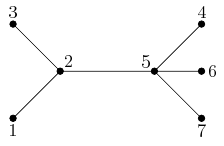
\includegraphics[]{hot.png}
	
	호텔을 세울 수 있는 위치는 다음과 같다: \{1, 3, 5\}, \{2, 4, 6\}, \{2, 4, 7\}, \{2, 6, 7\}, \{4, 6, 7\}
	
\end{problem}

